% Created 2025-04-02 Wed 16:21
% Intended LaTeX compiler: pdflatex
\documentclass[11pt]{article}
\usepackage[utf8]{inputenc}
\usepackage[T1]{fontenc}
\usepackage{graphicx}
\usepackage{longtable}
\usepackage{wrapfig}
\usepackage{rotating}
\usepackage[normalem]{ulem}
\usepackage{amsmath}
\usepackage{amssymb}
\usepackage{capt-of}
\usepackage{hyperref}
\author{victoria}
\date{\today}
\title{Jones Polynomial}
\hypersetup{
 pdfauthor={victoria},
 pdftitle={Jones Polynomial},
 pdfkeywords={},
 pdfsubject={},
 pdfcreator={Emacs 29.1.90 (Org mode 9.6.14)}, 
 pdflang={English}}
\begin{document}

\maketitle
The Jones polynomial associates a Laurent polynomial with integer coefficients to every knot and link. This polynomial is invariant under Reidemeister moves, making it a useful tool for distinguishing knots.

In order to define the Jones polynomial, we first need to define the Kauffman Bracket.

\section{The Kauffman Bracket}

The Kauffman bracket is a function from unoriented link diagrams in the oriented plane (or \(S^2\)) to Laurent polynomials with integer coefficients in an indeterminate \$A\$\$. It maps a diagram \(D\) to \(\langle D \rangle \in \mathbb{Z}[A^{-1}, A]\) and is characterized by:

,where \(\bigcirc\) is the unknot and \(D \sqcup \bigcirc\) consists of the diagram \(D\) along with an additional closed curve that does not cross itself or \(D\). The skein relation \((iii)\) expresses how the polynomial changes when resolving a crossing.

The bracket polynomial of a diagram with \(n\) crossings can be computed by resolving crossings recursively, reducing it to a sum of \(2^n\) crossing-free diagrams. If a diagram has \(c\) components and no crossings, its polynomial follows as \((-A^{-2} - A^2)^{c-1}\).

The ordering of crossing resolutions does not affect the final result, ensuring the well-defined nature of the Kauffman bracket. If an orientation-preserving homeomorphism of the plane is applied to the diagram, the polynomial remains unchanged. 

We will now analyze the effect of Reidemeister moves on the bracket polynomial.

\section{Effect of Reidemeister Moves}

If a diagram is changed by a \textbf{Type I Reidemeister} move, its bracket polynomial changes as follows:

\begin{equation}
    \langle \raisebox{-0.15cm}{\includegraphics[width=0.5cm]{reidemeister_I.pdf}} \rangle = (A(-A^{-2} - A^2) + A^{-1}) \langle D \rangle.
\end{equation}

This follows from an application of the skein relation. If the crossing were reversed, the formula remains the same except for an interchange of \(A\) and \(A^{-1}\). This symmetry results from rotating the skein relation by \(\pi/2\). If \(D'\) is the reflection of \(D\) (with all crossings flipped), then \(\langle D' \rangle\) is obtained by exchanging \(A\) and \(A^{-1}\) in \(\langle D \rangle\).

This lemma is used in subsequent calculations, including the bracket polynomial of a two-component link and a trefoil knot. For example:

\begin{equation}
    \langle \raisebox{-0.15cm}{\includegraphics[width=0.5cm]{two_component_link.pdf}} \rangle = A \langle \raisebox{-0.15cm}{\includegraphics[width=0.5cm]{resolved_1.pdf}} \rangle + A^{-1} \langle \raisebox{-0.15cm}{\includegraphics[width=0.5cm]{resolved_2.pdf}} \rangle = (-A^4 - A^{-4}).
\end{equation}

For the trefoil knot:

\begin{equation}
    \langle \raisebox{-0.15cm}{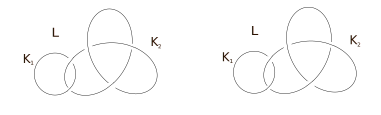
\includegraphics[width=0.5cm]{trefoil.pdf}} \rangle = A \langle \raisebox{-0.15cm}{\includegraphics[width=0.5cm]{resolved_1.pdf}} \rangle + A^{-1} \langle \raisebox{-0.15cm}{\includegraphics[width=0.5cm]{resolved_2.pdf}} \rangle = A(-A^4 - A^{-4}) + A^{-7} = (A^{-7} - A^{-3} - A^5).
\end{equation}
\end{document}
